\documentclass[a4paper]{article}
\usepackage{graphicx}
\usepackage{amsmath, amsfonts, geometry, float, listings, enumerate, multicol}
\usepackage{multicol, float, color, colortbl}
\usepackage{tikz, titlesec, parskip, pgfplots, filecontents}
\usepackage{hyperref}
\usepackage{amsmath}
\usepackage{tikz, titlesec, parskip}
\usepackage{tikz,pgfplots}
\usepackage[americanvoltages,fulldiodes,siunitx]{circuitikz}
\usetikzlibrary{shapes,arrows}
\usepackage{enumitem}

\titlespacing{\section}{0pt}{10pt}{0pt}
\titlespacing{\subsection}{0pt}{10pt}{0pt}
\titlespacing{\subsubsection}{0pt}{10pt}{0pt}

\usetikzlibrary{calc,patterns,through}
\newcommand{\arcangle}{%
	\mathord{<\mspace{-9mu}\mathrel{)}\mspace{2mu}}%
}

\renewcommand{\baselinestretch}{1.4}
 \geometry{
 a4paper,
 total={170mm,257mm},
 left=20mm,
 top=20mm,
 }
\usepackage{fancyhdr}
\usepackage{indentfirst}
\pagestyle{fancy}
\fancyhf{}
\rhead{\textbf{آمار و احتمال مهندسی}}
\lhead{\textbf{تمرین عملی سری اول}}
\cfoot{(\space \space \space \space \textbf{\thepage}  \space \space \space)}
\renewcommand{\headrulewidth}{1pt}
\renewcommand{\footrulewidth}{1pt}

 
\usepackage{xepersian}
\setlatintextfont{Times New Roman}
\settextfont{XB Niloofar}
\setdigitfont{XB Niloofar}
\DefaultMathsDigits

\makeatletter
\bidi@patchcmd{\@Abjad}{آ}{الف}
{\typeout{Succeeded in changing آ into الف}}
{\typeout{Failed in changing آ into الف}}
\makeatother
\PersianAlphs

\begin{document}
\begin{minipage}{0.6\textwidth}
\begin{bf}
\begin{center}
	به نام خدا\\
	\vspace{0.25cm}
	دانشگاه صنعتی شریف\\
	\vspace{0.25cm}
	دانشکده مهندسی برق\\
	\vspace{0.5cm}

\large
گروه دکتر یاسایی - آمار و احتمال مهندسی \\
نیم سال اول
۱۴۰۱-۱۴۰۰\\
\Large
\vspace{0.4cm}
تمرین عملی سری اول\\
\end{center}
\end{bf}
\normalsize
\end{minipage} \hfill
\begin{minipage}{0.35\textwidth}
\begin{flushleft}
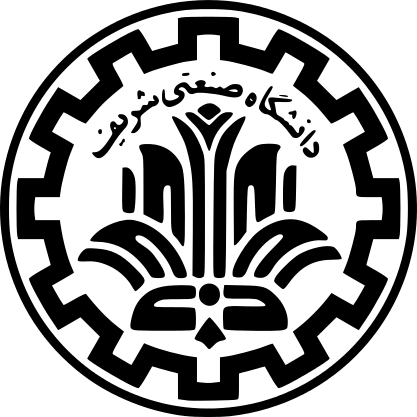
\includegraphics[width=0.6\textwidth]{Shariflogo.png}\\ \large
\end{flushleft}

 \end{minipage}
\\

\rule[0.1\baselineskip]{\textwidth}{1.5pt}

\large

\section*{
لطفاً به نکات زیر توجه بفرمایید:
}
\begin{enumerate}
	\item 
نتایج و پاسخ های خود را در یک فایل با فرمت zip به نام
\LR{HW$1$-Name-StudentNumber}
 در سایت  cw قرار دهید.
	\item 
کسب نمره کامل در هر سؤال مستلزم تحویل  \textbf{کدها} و \textbf{توضیحات} می‌باشد. 
\item 
برای سؤالات، باید روشی که استفاده کرده‌اید را توضیح  و نتایجی که گرفته‌اید را ارائه دهید. این توضیحات می‌تواند در یک فایل  pdf  و یا در یک فایل  ipynb باشد. 
\item 
کدهای خود را خوانا بنویسید و کامنت‌‌گذاری کنید. در plot های خود عنوان، label و خط‌کشی‌های مناسب را اضافه کنید.
\item
ابهام يا اشكالات خود را مي توانيد  از طریق
\href{https://t.me/Amirhosein_javadi}{@Amirhosein\_Javadi}
یا 
\href{mailto:javadiamirhosein.2000@gmail.com}{\LR{Javadiamirhosein.$2000$@gmail.com}}
مطرح نماييد.
\item 
کدهای شما تماماً باید توسط خودتان نوشته شده باشند. هرگونه استفاده از کد دیگران به هر شکل ممکن، تقلب محسوب می‌شود و نمره تمرین کامپیوتری جاری صفر خواهد شد. پس در هیچ صورت کدهای خود را برای دیگران ارسال نکنید.

\item 
مهلت تحویل:  
\end{enumerate}
\clearpage
\section{
متغیرهای تصادفی و تحقق‌هایش
}
در این سوال قصد داریم با نمونه‌برداری از متغیرهای تصادفی به یک هیستوگرام برسیم و با تفاوت بین این هیستوگرام و تابع احتمال متغیرهای تصادفی بیشتر آشنا شویم.
\begin{enumerate}
	\item 
فرض کنید:
	\begin{equation*}
		X_{1},X_{2},X_{3} = Bernoulli(0.6)
	\end{equation*}
از متغیر تصادفی‌های 
$ 	X_{1},X_{2},X_{3} $،
$ N = 10000 $
نمونه بردارید و $ Y $ را به شکل زیر تعیرف کنید.
	\begin{equation*}
	Y = X_{1}+X_{2}+X_{3}
	\end{equation*} 
حال هیستوگرام $ Y $ را رسم کنید. انتظار دارید این هیستوگرام متناظر با تابع احتمال  جه متغیر تصادفی با چه پارامترهایی است؟
	\item 
از متغیر تصادفی 
$ Poisson( \lambda=5) $،
$ N = 10000 $
نمونه ‌بردارید. هیستوگرام این نمونه‌‌ها و تابع جرم احتمال این متغیر تصادفی را در یک plot رسم کنید و با هم مقایسه کنید.
	\item 
از متغیر تصادفی 
	$ Exponential( \lambda=1) $،	
	$ N = 10000 $
نمونه ‌بردارید. آرایه‌ای به سایز $ N $ به صورت زیر تعریف کنید:
\begin{equation*}
	MyArray[i] = Average(samples[1:i])
\end{equation*}
سپس آرایه‌ی به دست آمده را در یک plot رسم کنید. انتظار دارید این آرایه به چه عددی میل کند؟ پارامتر‌های متغیر تصادفی را تغییر دهید و حدس خود را بیازمایید.
\end{enumerate}
\section{
سکه‌ی جادویی
}
سکه‌ای داریم که احتمال شیر آمدنش متناسب با معکوس تعداد پرتاب آن است! به این صورت که اگر بخواهیم
 $ n $
 پرتاب با سکه داشته باشیم، احتمال شیر آمدن سکه در هر پرتاب 
  $ \frac{4}{n} $
 است. هیستوگرم تعداد شیر آمده را برای 
 $ n = 10,100,1000,10000 $
 در چهار subplot رسم کنید. 


\section{
پارادوکس روز تولد
}
در این بخش قصد داریم با موضوع پارادوکس روز تولد بیشتر آشنا شویم. فرض کنید امیرحسین قصد دارد مهمانی برگزار کند و از $ n $ نفر دعوت کند. قسمت هیجان‌انگیز این مهمانی بازی‌ است که امیرحسین تدارک دیده‌است. امیرحسین از هر مهمان می‌خواهد که روز تولد خود را روی کاغذ بنویسد و به او بدهد. اگر حداقل دو نفر از مهمان‌‌ها متولد یک روز باشند امیرحسین  بازی را میبرد و مهمان‌ها باید پول سفر ‌امیرحسین به تور اروپا را بدهند. در غیر این صورت امیرحسین باید هزینه‌ی سفر‌ همه‌ی مهمان‌ها به ساری را بدهد. از آن‌جایی که امیرحسین باید به همه‌ی مهمان‌ها شام بدهد نمی‌خواهد تعداد مهمان‌‌ها را زیاد در نظر بگیرد. برای همین می‌خواهیم به امیرحسین کمک کنیم که با کمترین تعداد مهمان با احتمال بالایی بازی را ببرد و به تور اروپا برود. 
\begin{enumerate}
	\item
$ 10000 $ آزمایش انجام بدهید. در هر آزمایش قصد داریم تخمینی از $ n $ به دست بیاوریم. در هر آزمایش شروع به انتخاب تصادفی روز‌های سال کنید و زمانی که روزی را انتخاب کردید که قبلا هم انتخاب کرده بودید تعداد انتخاب‌‌هایی که تا آن مرحله انجام داده بودید را ثبت کنید. سپس هیستوگرامی از تعداد انتخاب‌های این $ 10000 $  آزمایش رسم کنید. 
	\item
حال احتمال پیروزی امیرحسین به ازای $ n $ مهمان را برای
	$ n = 1:365 $ 
را به دست بیاورید و رسم کنید. اگر امیرحسین بخواهد با احتمال
 $  \frac{1}{2}$
 برنده شود باید چند مهمان دعوت کند؟
\end{enumerate}
\end{document}
